\documentclass[12pt,a4paper,twoside]{report}
% -------------------------------------------------------------------- %
% Pacotes

\usepackage[utf8]{inputenc}
\usepackage[T1]{fontenc}
\usepackage[brazil]{babel}
\usepackage[fixlanguage]{babelbib}
\usepackage[pdftex]{graphicx}      % usamos arquivos pdf/png como figuras
\usepackage{setspace}              % espaçamento flexvel
\usepackage{indentfirst}           % indentação do primeiro parágrafo
\usepackage{makeidx}               % índice remissivo
\usepackage[nottoc]{tocbibind}     % acrescentamos a bibliografia/indice/conteudo no Table of Contents
\usepackage{courier}               % usa o Adobe Courier no lugar de Computer Modern Typewriter
\usepackage{type1cm}               % fontes realmente escaláveis
\usepackage{titletoc}
\usepackage{ucs}
\usepackage[font=small,format=plain,labelfont=bf,up,textfont=it,up]{caption}
\usepackage[usenames,svgnames,dvipsnames]{xcolor}
\usepackage[a4paper,top=2.54cm,bottom=2.0cm,left=2.0cm,right=2.54cm]{geometry} % margens
\usepackage{amsmath}

\usepackage[pdftex,plainpages=false,pdfpagelabels,pagebackref,colorlinks=true,citecolor=DarkGreen,
linkcolor=NavyBlue,urlcolor=DarkRed,filecolor=green,bookmarksopen=true]{hyperref} % links coloridos
\usepackage[all]{hypcap}                % soluciona o problema com o hyperref e capítulos
\usepackage[square,sort,nonamebreak,comma]{natbib}  % citação bibliográfica alpha
\fontsize{60}{62}\usefont{OT1}{cmr}{m}{n}{\selectfont}
\usepackage{upquote}                    % formata apóstrofes '
\usepackage{textcomp}

% Para formatar corretamente as URLs
\usepackage{url}
% -------------------------------------------------------------------- %
% Cabeçalhos similares ao TAOCP de Donald E. Knuth
\usepackage{fancyhdr}
\pagestyle{fancy}
\fancyhf{}
\renewcommand{\chaptermark}[1]{\markboth{\MakeUppercase{#1}}{}}
\renewcommand{\sectionmark}[1]{\markright{\MakeUppercase{#1}}{}}
\renewcommand{\headrulewidth}{0pt}

% -------------------------------------------------------------------- %
\graphicspath{{./imagens/}}        % caminho das figuras
\frenchspacing                     % arruma o espaço: id est (i.e.) e exempli gratia (e.g.)
\urlstyle{same}                    % URL com o mesmo estilo do texto e no mono-spaced
\makeindex                         % para o índice remissivo
\raggedbottom                      % para no permitir espaços extras no texto
\fontsize{60}{62}\usefont{OT1}{cmr}{m}{n}{\selectfont}
\cleardoublepage
\normalsize

% -------------------------------------------------------------------- %
% Cores para formatação de código
\usepackage{color}
\definecolor{vermelho}{rgb}{0.6,0,0} % para strings
\definecolor{verde}{rgb}{0.25,0.5,0.35} % para comentários
\definecolor{roxo}{rgb}{0.5,0,0.35} % para palavras-chaves
\definecolor{azul}{rgb}{0.25,0.35,0.75} % para strings
\definecolor{cinza-claro}{gray}{0.95}
% -------------------------------------------------------------------- %
% Opções de listagem usados para o código fonte
% Ref: http://en.wikibooks.org/wiki/LaTeX/Packages/Listings



\usepackage{listings}           % para formatar código-fonte (ex. em Java)


\lstset{ %
language=[Objective]Caml,  % seleciona a linguagem do código (aqui em lstlang0.sty
basicstyle=\footnotesize\ttfamily, % o tamanho da fonte usado no código
commentstyle=\color{verde}\bfseries,  % formatação de comentários
stringstyle=\color{azul},    % formatação de strings
upquote=true,
numbers=left,                   % onde colocar os números de linha
numberstyle=\tiny,  % o tamanho da fonte usada para a numeração das linhas
stepnumber=1,                   % o intervalo entre dois números de linhas. Se for 1, numera cada uma.
numbersep=5pt,                  % how far the line-numbers are from the code
showspaces=false,               % show spaces adding particular underscores
showstringspaces=false,         % underline spaces within strings
showtabs=false,                 % show tabs within strings adding particular underscores
keywordstyle=\color{roxo}\bfseries,
keywordstyle=[1]\color{roxo}\bfseries,
keywordstyle=[2]\color{verde}\bfseries,
%        keywordstyle=[3]\textbf,    %
%        keywordstyle=[4]\textbf,   \sqrt{\sqrt{}} %
frame=b,                   % adds a frame around the code
framerule=0.6pt,
tabsize=2,                      % sets default tabsize to 2 spaces
captionpos=t,                   % sets the caption-position to top
breaklines=true,                % sets automatic line breaking
breakatwhitespace=false,        % sets if automatic breaks should only happen at whitespace
escapeinside={\%*}{*)},         % if you want to add a comment within your code
backgroundcolor=\color[rgb]{1.0,1.0,1.0}, % choose the background color.
rulecolor=\color[rgb]{0.8,0.8,0.8},
extendedchars=true,
xleftmargin=10pt,
xrightmargin=10pt,
framexleftmargin=10pt,
framexrightmargin=10pt,
literate={â}{{\^{a}}}1  % para formatar corretamente os acentos do Português ao usar utf8
    {ê}{{\^{e}}}1
    {ô}{{\^{o}}}1
    {Â}{{\^{A}}}1
    {Ê}{{\^{E}}}1
    {Ô}{{\^{O}}}1
    {á}{{\'{a}}}1
    {é}{{\'{e}}}1
    {í}{{\'{i}}}1
    {ó}{{\'{o}}}1
    {ú}{{\'{u}}}1
    {Á}{{\'{A}}}1
    {É}{{\'{E}}}1
    {Í}{{\'{I}}}1
    {Ó}{{\'{O}}}1
    {Ú}{{\'{U}}}1
    {à}{{\`{a}}}1
    {À}{{\`{A}}}1
    {ã}{{\~{a}}}1
    {õ}{{\~{o}}}1
    {Ã}{{\~{A}}}1
    {Õ}{{\~{O}}}1
    {ç}{{\c{c}}}1
    {Ç}{{\c{C}}}1
    {ü}{{\"u}}1
    {Ü}{{\"U}}1
}

\renewcommand{\lstlistingname}{Listagem}
\renewcommand{\lstlistlistingname}{Lista de Listagens}

% Definição de novos estilos
\lstdefinestyle{Bash}
    {language=bash,frame=single,numbers=none,basicstyle=\footnotesize\ttfamily,
     morekeywords={cp,mkdir,sudo,tar}}

% Definição de novos ambientes
\lstnewenvironment{terminal}
  {\lstset{style=Bash}}
  {}

\lstnewenvironment{ocaml}
  {\lstset{basicstyle=\scriptsize\ttfamily,
           frame=single,
           frameround=tttt,
           framerule=2pt,
           numbers=none,
           rulecolor=\color{Salmon}}}
  {}

\lstnewenvironment{xml}
   {\lstset{language=XML,frame=single,numbers=none}}
   {}

\lstnewenvironment{interprete}
  {\lstset{frame=single,
            frameround=tttt,
            numbers=none,
            basicstyle=\ttfamily,
            framerule=2pt,
            rulecolor=\color{CadetBlue}}}
  {}
% Formata o caption da listagem
% \DeclareCaptionFont{blue}{\color{blue}}

% \captionsetup[lstlisting]{singlelinecheck=false, labelfont={blue}, textfont={blue}}
\usepackage{caption}
\DeclareCaptionFont{white}{\color{white}}
\DeclareCaptionFormat{listing}{\colorbox[cmyk]{0.43, 0.35, 0.35,0.01}{\parbox{\textwidth}{\hspace{15pt}#1#2#3}}}
\captionsetup[lstlisting]{format=listing,labelfont=white,textfont=white, singlelinecheck=false, margin=0pt, font={bf,footnotesize}}

\newcommand{\ListingsPath}{./codigos}
% Inclui o nome do arquivo como Caption
\newcommand{\filelisting}[2][]{%
    \lstinputlisting[caption={\texttt{\detokenize{#2}}},#1]{\ListingsPath/#2}%
}

% ---------------------------------------------------------------------------- %

% ---------------------------------------------------------------------------- %

\title{Construção de um compilador de Lua para Parrot Virtual Machine usando Objective Caml}
\date{}
\author{Guilherme Pacheco de Oliveira \\
\texttt{\small \url{guilherme.061@gmail.com}}
\vspace{1cm} \\
Faculdade de Computação \\
Universidade Federal de Uberlândia
}
\date{\today}

%\includeonly{cap-clojure,magical,short}
\begin{document}
  \maketitle
% -------------------------------------------------------------------- %
% Listas de figuras, tabelas e códigos criadas automaticamente
\listoffigures
\listoftables
\lstlistoflistings
% -------------------------------------------------------------------- %

% -------------------------------------------------------------------- %
% Sumário
\tableofcontents

% Capítulos do trabalho

% cabeçalho para as páginas de todos os capítulos
\fancyhead[RE,LO]{\thesection}

%\singlespacing              % espaçamento simples
\setlength{\parskip}{0.15in} % espaçamento entre paragráfos

\chapter{Introdução}
Este documento tem como intenção documentar todo o processo de construção de um compilador para a linguagem de programação Lua para a máquina virtual Parrot utilizando Objective OCaml.

A intenção é cobrir desde os primeiros passos, como instalação das ferramentas até conceitos de compiladores, implementações em OCaml e detalhes técnicos. Dessa forma, espera-se que um leitor seja capaz de replicar os resultados.

O Sistema Operacional utilizado é OS X El Capitain 10.11.6

\chapter{Instalação dos componentes}
\section{Homebrew}
Homebrew é um gerenciador de pacotes para Mac OS X, escrito em Ruby, e
é responsável por instalar pacotes nos diretórios adequados e fazer
adequadamente a configuração desses pacotes, instalá-lo facilita todo
o processo de instalação dos componentes necessários.

Para instalar o homebrew basta digitar no terminal:

\begin{terminal}
$ /usr/bin/ruby -e "\$(curl -fsSL https://raw.githubusercontent.com/Homebrew/install/master/install)"
\end{terminal}


\section{Lua}
\subsection{Instalação e Teste}
Para instalar Lua através do homebrew, basta digitar no terminal:
\begin{terminal}
$ brew install lua
\end{terminal}
Resultado:
\begin{figure}[!ht]
\centering
\caption{Instalando e testando LUA}
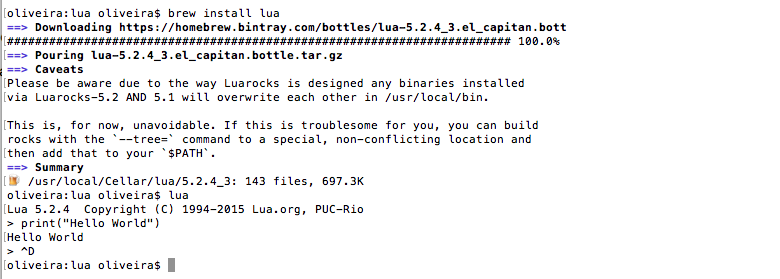
\includegraphics[scale=0.27]{imagens/brew-lua.png}
\end{figure}
\subsection{Informações sobre a linguagem Lua}
A principal referência para Lua é a documentação em seu site oficial [1].
Lua é uma linguagem de programação de extensão, projetada para dar suporte à outras linguagens de programação procedimental e planejada para ser usada como uma linguagem de script leve e facilmente embarcável, é implementada em C.



\section{Ocaml}
\subsection{Instalação e Teste}
Novamente através do homebrew, basta digitar:
\begin{terminal}
$ brew install ocaml
\end{terminal}
Resultado:
\begin{figure}[!ht]
\centering
\caption{Instalando e testando OCaml}
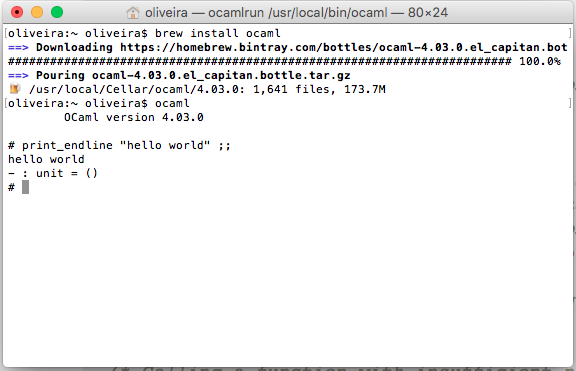
\includegraphics[scale=0.27]{imagens/brew-ocaml.png}
\end{figure}
\subsection{Informações sobre a linguagem OCaml}
A documentação oficial do OCaml [2] possui manuais, licenças, documentos e algumas dicas sobre como programar adequadamente na linguagem.
OCaml é uma linguagem de programação funcional, imperativa e orientada à objetos.

\section{Parrot Virtual Machine}

\subsection{Instalação e Teste}
Digitar no Terminal:
\begin{terminal}
$ brew install parrot
\end{terminal}
Resultado:
\begin{figure}[!ht]
\centering
\caption{Instalando e testando Parrot}
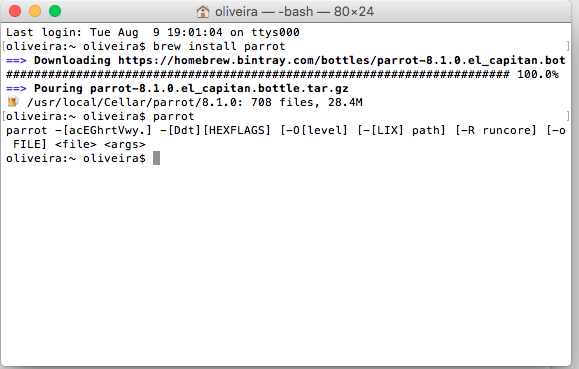
\includegraphics[scale=0.27]{imagens/brew-parrot.png}
\end{figure}
\subsection{Informações sobre a Parrot Virtual Machine}
A máquina virtual Parrot é utilizada principalmente para linguagens dinâmicas como Perl, Python, Ruby e PHP, seu design
foi originalmente feito para trabalhar com a versão 6 de Perl, mas seu uso foi expandido como uma maquina virtual dinâmica
e de proposito geral, apta a lidar com qualquer linguagem de programação de alto nível. [3]

Parrot pode ser programada em diversas linguagens, os dois mais utilizados são:
Parrot Assembly Language (PASM): É a linguagem de mais baixo nível utilizada pela Parrot, muito similar a um assembly tradicional.
Parrot Intermediate Representation(PIR): De mais alto nível que PASM, também um pouco mais facil de se utilizar e mais utilizada.

Fazendo alguns testes com PASM e PIR:
\lstinputlisting[caption={Output Simples em Parrot Assembly Language}]{codigos/parrot/news.pasm}
Para executar o código:
\begin{terminal}
$ parrot news.pasm
\end{terminal}

\lstinputlisting[caption={Output Simples em Parrot Intermediate Representation}]{codigos/parrot/hello.pir}
Para executar o código:
\begin{terminal}
$ parrot hello.pir
\end{terminal}

Os arquivos PASM e PIR são convertidos para Parrot Bytecode (PBC) e somente então são executados pela máquina virutal, é possível obter o arquivo .pbc através comando:
\begin{terminal}
$ parrot -o output.pbc input.pasm
\end{terminal}

De acordo com a documentação oficial, o Compilador Intermediário de Parrot é capaz de traduzir códigos PIR para PASM através do comando:
\begin{terminal}
$ parrot -o output.pasm input.pir
\end{terminal}
Mas essa execução resultou em um código bytecode invés do assembly.

Apesar da documentação oficial enfatizar que PIR é mais utilizado e mais recomendado para o desenvolvimento de compiladores para Parrot, o alvo será a linguagem Assembly PASM.

\subsection{Parrot Assembly Language (PASM)}
A linguagem PASM é muito similar a um assembly tradicional, com exceção do fato de que algumas instruções permitem o acesso a algumas funções dinâmicas de alto nível do sistema Parrot.

Parrot é uma maquina virtual baseada em registradores, há um número ilimitado de registradores que não precisam ser instanciados antes de serem utilizados, a maquina virtual se certifica de criar os registradores de acordo com a sua necessidade,
tal como fazer a reutilização e se livrar de registradores que não estão mais sendo utilizados, todos os registradores começam com o símbolo "\$" e existem 4 tipos de dados, cada um com suas regras:


Strings: Registradores de strings começam com um S, por exemplo: "\$S10" \\
Inteiros: Registradores de inteiros começam com um I, por exemplo: "\$I10" \\
Número: Registradores de números de ponto flutuante, começam com a letra N, por exemplo: "\$N10" \\
PMC: São tipos de dados utilizados em orientação a objetos, podem ser utilizados para guardar vários tipos de dados, começam com a letra P, por exemplo: "\$P10" \\
\\
Para mais referêcias sobre PASM, consultar [4], [7] para os opcodes e [8] para exemplos.

\subsection{Parrot Intermediate Representation (PIR)}
A maior dos compiladores possuem como alvo o PIR, inclusive o que será
utilizado para estudar qual o comportamento um compilador deve ter ao
gerar o assembly.
A própria máquina virtual Parrot possui um módulo intermediário capaz
de interpretar a linguagem PIR e gerar o bytecode ou o próprio
assembly (PASM), além disso, existem compiladores capaz de realizar a
mesma tarefa.

PIR é de nível mais alto que assembly mas ainda muito próximo do nível
de máquina, o principal benefício é a facilidade em programar em PIR
em comparação com a programação em PASM, além disso, ela foi feita
para compiladores de linguagens de alto nível gerarem código PIR para
trabalhar com a maquina Parrot.
Mais informações sobre PIR e sua sintaxe podem ser encontradas em [5].

\chapter{Compilação de Código Ruby para Parrot Intermediate Representation (PIR)}
O compilador que será utilizado será o Cardinal [6], é um compilador
da linguagem Ruby para a máquina virtual Parrot capaz de gerar código
o código intermediário (PIR) como saída.

A documentação do compilador é simples e clara, para baixar o
compilador basta digitar no terminal:
\begin{terminal}
$ git clone git://github.com/parrot/cardinal.git
\end{terminal}
Entre as várias opções de instalação, é possível faze-la utilizando do
próprio parrot, para isso basta entrar na pasta onde foi baixado o
Cardinal e digitar:
\begin{terminal}
$ winxed setup.winxed build
\end{terminal}

Para compilar é necessário estar na pasta de instalação e o comando é:
\begin{terminal}
$ parrot cardinal.pbc [arquivo].rb
\end{terminal}
Sendo o arquivo o diretório do arquivo Ruby que se deseja executar,
para gerar o PIR o comando é:
\begin{terminal}
$ parrot cardinal.pbc -o [output].pir --target=pir [arquivo].rb
\end{terminal}
Sendo output o diretório onde será salvo o arquivo PIR.

\subsubsection{Exemplo}
\lstinputlisting[caption={Programa nano 01 em Ruby}]{codigos/ruby/nano01.rb}
Compilação do Código Ruby:
\begin{terminal}
$ parrot /Users/oliveira/cardinal/cardinal/cardinal.pbc -o
../parrot/nano01.pir --target=pir nano01.rb
\end{terminal}
\lstinputlisting[caption={Programa nano 01 em PIR}]{codigos/parrot/nano01.pir}

A compilação dos programas Ruby não foi bem sucedida para todos os programas, além disso, programas que utilizavam a linha de código a seguir, que é utilizada para pegar dados do usuário, compilavam mas não funcionavam na máquina virtual.
\begin{terminal}
input = gets.chomp
\end{terminal}


\chapter{Códigos LUA e Parrot Assembly (PASM)}

Os códigos PASM dessa seção foram feitos manualmente, não foram utilizados compiladores para esse fim.

\subsection{Nano Programas}
\subsubsection{Nano 01}
\lstinputlisting[caption={Programa nano 01 em Lua}]{codigos/lua/nano01.lua}
\lstinputlisting[caption={Programa nano 01 em PASM}]{codigos/parrot/nano01.pasm}

\subsubsection{Nano 02}
\lstinputlisting[caption={Programa nano 02 em Lua}]{codigos/lua/nano02.lua}
\lstinputlisting[caption={Programa nano 02 em PASM}]{codigos/parrot/nano02.pasm}

\subsubsection{Nano 03}
\lstinputlisting[caption={Programa nano 03 em Lua}]{codigos/lua/nano03.lua}
\lstinputlisting[caption={Programa nano 03 em PASM}]{codigos/parrot/nano03.pasm}

\subsubsection{Nano 04}
\lstinputlisting[caption={Programa nano 04 em Lua}]{codigos/lua/nano04.lua}
\lstinputlisting[caption={Programa nano 04 em PASM}]{codigos/parrot/nano04.pasm}

\subsubsection{Nano 05}
\lstinputlisting[caption={Programa nano 05 em Lua}]{codigos/lua/nano05.lua}
\lstinputlisting[caption={Programa nano 05 em PASM}]{codigos/parrot/nano05.pasm}
Saída:
\begin{terminal}
2
\end{terminal}

\subsubsection{Nano 06}
\lstinputlisting[caption={Programa nano 06 em Lua}]{codigos/lua/nano06.lua}
\lstinputlisting[caption={Programa nano 06 em PASM}]{codigos/parrot/nano06.pasm}
Saída:
\begin{terminal}
-1
\end{terminal}

\subsubsection{Nano 07}
\lstinputlisting[caption={Programa nano 07 em Lua}]{codigos/lua/nano07.lua}
\lstinputlisting[caption={Programa nano 07 em PASM}]{codigos/parrot/nano07.pasm}
Saída:
\begin{terminal}
1
\end{terminal}

\subsubsection{Nano 08}
\lstinputlisting[caption={Programa nano 08 em Lua}]{codigos/lua/nano08.lua}
\lstinputlisting[caption={Programa nano 08 em PASM}]{codigos/parrot/nano08.pasm}
Saída:
\begin{terminal}
1
\end{terminal}

\subsubsection{Nano 09}
\lstinputlisting[caption={Programa nano 09 em Lua}]{codigos/lua/nano09.lua}
\lstinputlisting[caption={Programa nano 09 em PASM}]{codigos/parrot/nano09.pasm}
Saída:
\begin{terminal}
1
\end{terminal}

\subsubsection{Nano 10}
\lstinputlisting[caption={Programa nano 10 em Lua}]{codigos/lua/nano10.lua}
\lstinputlisting[caption={Programa nano 10 em PASM}]{codigos/parrot/nano10.pasm}
Saída:
\begin{terminal}
0
\end{terminal}

\subsubsection{Nano 11}
\lstinputlisting[caption={Programa nano 11 em Lua}]{codigos/lua/nano11.lua}
\lstinputlisting[caption={Programa nano 11 em PASM}]{codigos/parrot/nano11.pasm}
Saída:
\begin{terminal}
3
5
\end{terminal}

\subsubsection{Nano 12}
\lstinputlisting[caption={Programa nano 12 em Lua}]{codigos/lua/nano12.lua}
\lstinputlisting[caption={Programa nano 12 em PASM}]{codigos/parrot/nano12.pasm}
Saída:
\begin{terminal}
0
0
0
0
\end{terminal}

\subsection{Micro Programas}
\subsubsection{Micro 01}
\lstinputlisting[caption={Programa micro 01 em Lua}]{codigos/lua/micro01.lua}
\lstinputlisting[caption={Programa Micro 01 em PASM}]{codigos/parrot/micro01.pasm}
\begin{terminal}
Tabela de Conversao: Celsius -> Fahrenheit
Digite a Temperatura em Celsius: 20
A nova temperatura e: 68 graus F.
\end{terminal}

\subsubsection{Micro 02}
\lstinputlisting[caption={Programa micro 02 em Lua}]{codigos/lua/micro02.lua}
\lstinputlisting[caption={Programa Micro 02 em PASM}]{codigos/parrot/micro02.pasm}
\begin{terminal}
Digite o primeiro numero: 10
Digite o segundo numero: 20
o segundo numero e maior que o primeiro numero
Digite o primeiro numero: 20
Digite o segundo numero: 10
o primeiro numero e maior que o segundo numero
\end{terminal}

\subsubsection{Micro 03}
\lstinputlisting[caption={Programa micro 03 em Lua}]{codigos/lua/micro03.lua}
\lstinputlisting[caption={Programa Micro 03 em PASM}]{codigos/parrot/micro03.pasm}
\begin{terminal}
Digite um numero: 5
O numero nao esta no intervalo entre 100 e 200

Digite um numero: 150
O numero esta no intervalo entre 100 e 200

Digite um numero: 201
O numero nao esta no intervalo entre 100 e 200
\end{terminal}

\subsubsection{Micro 04}
\lstinputlisting[caption={Programa micro 04 em Lua}]{codigos/lua/micro04.lua}
\lstinputlisting[caption={Programa Micro 04 em PASM}]{codigos/parrot/micro04.pasm}
\begin{terminal}
Digite um numero: 50
Digite um numero: 50
Digite um numero: 50
Digite um numero: 50
Digite um numero: 50
Ao total foram digitados 5 numeros no intervalo entre 10 e 150.

Digite um numero: 02
Digite um numero: 03
Digite um numero: 25
Digite um numero: 60
Digite um numero: 160
Ao total foram digitados 2 numeros no intervalo entre 10 e 150.
\end{terminal}

\subsubsection{Micro 05}
\lstinputlisting[caption={Programa micro 05 em Lua}]{codigos/lua/micro05.lua}
\lstinputlisting[caption={Programa Micro 05 em PASM}]{codigos/parrot/micro05.pasm}
\begin{terminal}
H - Homem ou M - Mulher: H
H - Homem ou M - Mulher: M
H - Homem ou M - Mulher: H
H - Homem ou M - Mulher: M
H - Homem ou M - Mulher: M
Foram inseridos 2 homens
Foram inseridas 3 mulheres
\end{terminal}

\subsubsection{Micro 06}
\lstinputlisting[caption={Programa micro 06 em Lua}]{codigos/lua/micro06.lua}
\lstinputlisting[caption={Programa Micro 06 em PASM}]{codigos/parrot/micro06.pasm}
\begin{terminal}
Digite um numero de 1 a 5: 3
Tres
\end{terminal}

\subsubsection{Micro 07}
\lstinputlisting[caption={Programa micro 07 em Lua}]{codigos/lua/micro07.lua}
\lstinputlisting[caption={Programa Micro 07 em PASM}]{codigos/parrot/micro07.pasm}
\begin{terminal}
Digite um numero: 5
Positivo!
Deseja finalizar? (S/N): N
Digite um numero: -5
Negativo!
Deseja finalizar? (S/N): N
Digite um numero: 0
Zero!
Deseja finalizar? (S/N): S
\end{terminal}

\subsubsection{Micro 08}
\lstinputlisting[caption={Programa micro 08 em Lua}]{codigos/lua/micro08.lua}
\lstinputlisting[caption={Programa Micro 08 em PASM}]{codigos/parrot/micro08.pasm}
\begin{terminal}
Digite um numero: 50
O numero 50 e maior que 10.
Digite um numero: 5
O numero 5 e menor que 10.
Digite um numero: 0
O numero 0 e menor que 10.
\end{terminal}

\subsubsection{Micro 09}
\lstinputlisting[caption={Programa micro 09 em Lua}]{codigos/lua/micro09.lua}
\lstinputlisting[caption={Programa Micro 09 em PASM}]{codigos/parrot/micro09.pasm}
\begin{terminal}
Digite o preco: 10
Digite a venda: 10
O novo preco e: 11

Digite o preco: 40
Digite a venda: 600
O novo preco e: 46

Digite o preco: 90
Digite a venda: 1500
O novo preco e: 72
\end{terminal}

\subsubsection{Micro 10}
\lstinputlisting[caption={Programa micro 10 em Lua}]{codigos/lua/micro10.lua}
\lstinputlisting[caption={Programa Micro 10 em PASM}]{codigos/parrot/micro10.pasm}
\begin{terminal}
Digite um numero: 5
O fatorial de 5 e: 120
\end{terminal}

\subsubsection{Micro 11}
\lstinputlisting[caption={Programa micro 11 em Lua}]{codigos/lua/micro11.lua}
\lstinputlisting[caption={Programa Micro 11 em PASM}]{codigos/parrot/micro11.pasm}
\begin{terminal}
Digite um numero: 5
Positivo

Digite um numero: -5
Negativo

Digite um numero: 0
Zero
\end{terminal}

\chapter{Analisador Léxco}
\section{Análise Léxica}

A Análise Léxica tem como principal objetivo facilitar o entedimento do programa para as análises subsequentes do compilador. Essa análise poderia ser feita juntamente com a análise sintática, mas é feita separada por motivos de eficiência, modularização (facilita manutenção e alterações futuras) e por tradição, as linguagens geralmente são criadas com módulos separados para análise léxica e sintática.

As expressões para a análise geralmente são escritas em expressões regulares, assim, os analisadores léxicos são criados como um automato finito deterministico.

Um Analisador Léxico tem como input uma string correspondente a todo o código digitado, essa string é separada em uma lista de caracteres que subsequentemente é separada em tokens. Após a separação em tokens, é trabalho do analisador verificar a corretude léxica do código bem como rotular corretamente cada token reconhecido.

\section{Analisador Manual}
\subsection{Linguagem a ser interpretada}
A linguagem a ser interpretada é uma linguagem simples que reconhece algumas palavras reservadas básicas de todas as linguagens de programação, como: print, if, then, else e comandos como atribuição, soma, subtração e multiplicação, além de reconhecer identificadores e números inteiros, todas as linhas devem ser terminadas com um ponto e vírgula, um exemplo de um programa nessa linguagem:

\begin{terminal}
b := 2;
a := 1 + b;
print (a * b);
if1 := a - 2;
if2 := b + 3;
if if1 > 0
then print(if1);
else print(if2);
\end{terminal}


\subsection{Autômato reconhecedor da linguagem}
O autômato capaz de interpretar a linguagem é um autômato do tipo M = (ALF, Q, d, qo, F), onde F é o alfabeto de símbolos de entrada, Q são os estados possíveis do autômato, d é a função de transição, qo é o estado inicial e F é o conjunto de todos os estados finais do autômato.

ALF = o alfabeto de entrada é qualquer conjunto de palavras sobre o conjunto ASCII 2

Q = {inicio, p, pr, pri, prin, print, i, if, t, th, the, then, e, el, els, else, identificador, inteiro, abre-parentese, fecha-parentese, comparador, operador, dois-pontos, atribuicao, ponto-virgula, estado-morto}

qo = inicio

F = {print, if, then, else, identificador, inteiro, abre-parentese, fecha-parentese, comparador, operador, atribuicao, ponto-virgula}

d =
A função de transição será descrita na forma:
(estado atual, simbolo lido, proximo estado), todos as transições que não forem listadas dessa forma levam ao estado morto que invalida a palavra lida.

(inicio, 'p', p)

(inicio, 'i', i)

(inicio, 't', t)

(inicio, 'e', e)

(inicio, '(', abre-parentese)

(inicio, ')', fecha-parentese)

(inicio, '>', comparador)

(inicio, '+', '-', '*', operador)

(inicio, ':', dois-pontos)

(inicio, ';', ponto-virgula)

(inicio, '0'-'9', inteiro)

(inicio, 'a'-'z', 'A'-'Z' ou '\_', identificador)

(p, 'r', pr)

(p, 'a'-'z' exceto 'r' ou 'A'-'Z' ou '0'-'9', identificador)

(pr, 'i', pri)

(pr, 'a'-'z' exceto 'i' ou 'A'-'Z' ou '0'-'9', identificador)

(pri, 'n', prin)

(pri, 'a'-'z' exceto 'n' ou 'A'-'Z' ou '0'-'9', identificador)

(prin, 't', print)

(print, 'a'-'z' exceto 't' ou 'A'-'Z' ou '0'-'9', identificador)

(print, 'a'-'z' ou 'A'-'Z' ou '0'-'9', identificador)

(i, 'f', if)

(i, 'a'-'z' exceto 'f', 'A'-'Z' ou '0'-'9', identificador)

(if, 'a'-'z' ou 'A'-'Z' ou '0'-'9', identificador)

(e, 'l', el)

(e, 'a'-'z' ou 'A'-'Z' ou '0'-'9', identificador)

(el, 's', els)

(el, 'a'-'z' ou 'A'-'Z' ou '0'-'9', identificador)

(els, 'e', else)

(els, 'a'-'z' ou 'A'-'Z' ou '0'-'9', identificador)

(else, 'a'-'z' ou 'A'-'Z' ou '0'-'9', identificador)

(t,'h', th)

(t, 'a'-'z' ou 'A'-'Z' ou '0'-'9', identificador)

(th, 'e', the)

(th, 'a'-'z' ou 'A'-'Z' ou '0'-'9', identificador)

(the, 'n', then)

(the, 'a'-'z' ou 'A'-'Z' ou '0'-'9', identificador)

(then, 'a'-'z' ou 'A'-'Z' ou '0'-'9', identificador)

(identificador, 'a'-'z' ou 'A'-'Z' ou '0'-'9', identificador)

(inteiro, '0'-'9', inteiro)

(dois-pontos, '=', atribuicao)

(atribuicao, - , estado-morto)

(abre-parentese, -, estado-morto)

(fecha-parentese, -, estado-morto)

(comparador, -, estado-morto)

(operador, -, estado-morto)

(ponto-virgula, -, estado-morto)

\subsection{Implementação}
\subsubsection{Convenções}
Para facilitar a escrita e o entendimento do código, os estados descritos acima foram codificados como números inteiros da seguinte forma:

\begin{center}
\begin{tabular} {| l | c |}
\hline
Nome do Estado & Inteiro Correspondente \\
inicio & 0 \\
p & 1 \\
pr & 2 \\
pri & 3 \\
prin & 4 \\
print & 5 \\
i & 6 \\
if & 7 \\
t & 8 \\
th & 9 \\
the & 10 \\
then & 11 \\
e & 12 \\
el & 13 \\
els & 14 \\
else & 15 \\
identificador & 16 \\
inteiro & 17 \\
abre-parentese & 18 \\
fecha-parentese & 19 \\
comparador & 20 \\
operador & 21 \\
dois-pontos & 22 \\
ponto-virgula & 23 \\
branco & 24 \\
atribuicao & 25 \\
estado-morto & -1 \\
\hline
\end{tabular}
\end{center}

\subsubsection{Código do Autômato}
Abaixo se encontram as modificações feitas no código já fornecido do analisador léxico para que ele pudesse reconhecer a linguagem descrita mais acima:

\lstinputlisting[caption={Automato reconhecedor da linguagem descrita}]{codigos/analisadorLexico/alteracoes.ml}

\subsubsection{Reconhecimento do Código}
Para demonstrar o funcionamento do autômato, será feita a entrada de um exemplo de programa, que foi especificado anteriormente e está novamente listado abaixo:

\begin{terminal}
b := 2;
a := 1 + b;
print (a * b);
if1 := a - 2;
if2 := b + 3;
if if1 > 0
then print(if1);
else print(if2);
\end{terminal}

Para iniciar o Ocaml, ler o arquivo e interpretar um código, os seguintes comandos devem ser especificados no terminal:
\begin{terminal}
rlwrap ocaml
#use "dfalexer.ml";;
lexico "comando";;

exit 0;;
\end{terminal}

Para testar o exemplo, será feita a entrada do programa como uma única string:
\begin{terminal}
#use "dfalexer.ml";;
lexico "b := 2;\na := 1 + b;\nprint (a * b);\nif1 := a - 2;\nif2 := b + 3;\nif if1 > 0\nthen print(if1);\nelse print(if2);";;

- : token list =
[Id "b"; Branco; Atribuicao; Branco; Int "2"; PontoVirgula; Branco; Id "a";
 Branco; Atribuicao; Branco; Int "1"; Branco; Operador "+"; Branco; Id "b";
 PontoVirgula; Branco; Print; Branco; AbreParentese; Id "a"; Branco;
 Operador "*"; Branco; Id "b"; FechaParentese; PontoVirgula; Branco;
 Id "if1"; Branco; Atribuicao; Branco; Id "a"; Branco; Operador "-"; Branco;
 Int "2"; PontoVirgula; Branco; Id "if2"; Branco; Atribuicao; Branco;
 Id "b"; Branco; Operador "+"; Branco; Int "3"; PontoVirgula; Branco; If;
 Branco; Id "if1"; Branco; Comparador ">"; Branco; Int "0"; Branco; Then;
 Branco; Print; AbreParentese; Id "if1"; FechaParentese; PontoVirgula;
 Branco; Else; Branco; Print; AbreParentese; Id "if2"; FechaParentese;
 PontoVirgula; EOF]
\end{terminal}

Para verificar a corretude do automato, testarei também com um exemplo negativo, por exemplo, colocando um @ no meio da string de teste:

\begin{terminal}
#use "dfalexer.ml";;
lexico "b := 2;\na := 1 @ + b;\nprint (a * b);\nif1 := a - 2;\nif2 := b + 3;\nif if1 > 0\nthen print(if1);\nelse print(if2);";;

Exception: Failure "Erro lexico: caracter desconhecido @".
\end{terminal}

\section{Analisador com Ocamllexer}
\subsection{Convenções Léxicas da Linguagem Lua}
Na documentação oficial da Linguagem Lua, as convenções léxicas podem ser encontradas na Seção 3.1.

Lua ignora espaços brancos, novas linhas e comentários entre elementos léxicos (tokens).

Nomes (identificadores) em Lua podem ser strings de letras, digitos e underscore, não podendo começar com um digito. Identificadores são utilizados para rotular variáveis, tabelas e rótulos.

A Linguagem possui as seguintes palavras reservadas:

\begin{center}
\begin{tabular} {| c | c | c | c | c | c | }
\hline
and & break & do & else & elseif & end \\
\hline
false & for & function & goto & if & in \\
\hline
local & nil & not & or & repeat & return \\
\hline
then & true & until & while & &\\
\hline
\end{tabular}
\end{center}

Lua é caso sensitivo, and é uma palavra reservada, porém AND, And, aNd, etc... podem ser utilizadas como identificadores. Por convenção, identificadores que começam com underscore e são seguidos por letras maiúsculas (como \_VERSION) são variáveis utilizadas pela linguagem

São outros tokens reconhecidos pela linguagem:


\begin{center}
\begin{tabular} {| c | c | c | c | c | c | c |}
\hline
+ & - & * & / & \% & \^{} & \# \\
\hline
== & \~{}= & <= & >= & < & > & =\\
\hline
( & ) & \{ & \} & [ & ] & ::\\
\hline
; & : & , & . & .. & ... & \\
\hline
\end{tabular}
\end{center}

Strings podem ser limitadas por aspas simples ou duplas e pode conter qualquer caractere de escape contido no C:

\begin{terminal}
 '\a', '\b', '\f', '\n', '\r', '\t', '\v', '\\', '\"' e '\''
\end{terminal}

Strings em Lua também podem ser criadas utilizando uma notação de colchetes, em n níveis, as seguintes strings são aceitas em lua:

\begin{terminal}
 [[teste]] [=[teste]=] [==[teste]==] ...
\end{terminal}

Uma constante numérica pode ser escrita com uma parte fracionária opcional, marcada por 'e' ou 'E'. Lua também aceita constantes hexadecimais, que começam com '0x' ou '0X', e aceitam um complemento binário que vem após um 'p' ou 'P', as seguintes constantes numéricas são aceitas:

\begin{terminal}
 3     3.0     3.1416     314.16e-2     0.31416E1
 0xff  0x0.1E  0xA23p-4   0X1.921FB54442D18P+1
\end{terminal}

Um comentário começa com -- fora de uma string, se após os dois hífens não vier um colchete, o comentário é de uma linha, caso contrário, o comentário segue até encontrar um colchete fechando o comentário.

\subsection{Implementação}

A implementação foi feita utilizando Ocaml Lex, uma ferramente própria para desenvolvimento de analisadores léxicos utilizando autômatos finitos, o código implementado está a seguir.

\lstinputlisting[caption={Arquivo do Reconhecedor léxico de Lua}]{codigos/analisadorLexico/lexer/lualexer.mll}

Além disso, é utilizado o arquivo carregador, fornecido em aula, para que se possa testar corretamente o analisador.

\lstinputlisting[caption={Carregador}]{codigos/analisadorLexico/lexer/carregador.ml}

\subsection{Testes}

Para compilar e executar corretamente o Analisador Léxico os seguintes comandos devem ser utilizados:

\begin{terminal}
ocamllex lualexer.mll
ocamlc lualexer.ml

rlwrap ocaml
#use "carregador.ml";;
\end{terminal}

Para testar todos os tokens, foi escrito o seguinte arquivo de teste:

\lstinputlisting[caption={Teste de Tokens}]{codigos/analisadorLexico/lexer/teste.lua}

Que fornece o seguinte resultado:

\begin{terminal}
# lex "teste.lua";;
- : Lualexer.tokens list =
[Lualexer.INT 2; Lualexer.OPERADOR "+"; Lualexer.INT 2; Lualexer.INT 2;
 Lualexer.OPERADOR "-"; Lualexer.INT 2; Lualexer.INT 2;
 Lualexer.OPERADOR "*"; Lualexer.INT 2; Lualexer.INT 2;
 Lualexer.OPERADOR "/"; Lualexer.INT 2; Lualexer.INT 2;
 Lualexer.OPERADOR "%"; Lualexer.INT 2; Lualexer.INT 2;
 Lualexer.OPERADOR "^"; Lualexer.INT 2; Lualexer.INT 2;
 Lualexer.COMPARADOR "=="; Lualexer.INT 2; Lualexer.INT 2;
 Lualexer.COMPARADOR "<="; Lualexer.INT 2; Lualexer.INT 2;
 Lualexer.COMPARADOR ">="; Lualexer.INT 2; Lualexer.INT 2;
 Lualexer.COMPARADOR "<"; Lualexer.INT 2; Lualexer.INT 2;
 Lualexer.COMPARADOR ">"; Lualexer.INT 2; Lualexer.INT 1234;
 Lualexer.INT 23908423; Lualexer.INT 123124; Lualexer.INT 1032490;
 Lualexer.INT 324932; Lualexer.INT 3294; Lualexer.ID "identificador";
 Lualexer.ID "m"; Lualexer.ID "n"; Lualexer.ID "i"; Lualexer.ID "j";
 Lualexer.ID "k"; Lualexer.ID "l"; Lualexer.QUADRADO; Lualexer.DOISPONTOS;
 Lualexer.DOISDOISPONTOS; Lualexer.PONTOEVIRGULA; Lualexer.VIRGULA;
 Lualexer.PONTO; Lualexer.PONTOPONTO; Lualexer.PONTOPONTOPONTO;
 Lualexer.ABREPARENTESE; Lualexer.FECHAPARENTESE; Lualexer.ABRECOLCHETE;
 Lualexer.FECHACOLCHETE; Lualexer.ABRECHAVES; Lualexer.FECHACHAVES;
 Lualexer.ATRIBUICAO; Lualexer.AND; Lualexer.BREAK; Lualexer.DO;
 Lualexer.ELSE; Lualexer.ELSEIF; Lualexer.END; Lualexer.FALSE; Lualexer.FOR;
 Lualexer.FUNCTION; Lualexer.GOTO; Lualexer.IF; Lualexer.IN; Lualexer.LOCAL;
 Lualexer.NIL; Lualexer.NOT; Lualexer.OR; Lualexer.REPEAT; Lualexer.RETURN;
 Lualexer.THEN; Lualexer.TRUE; Lualexer.UNTIL; Lualexer.WHILE;
 Lualexer.STRING "hello world"; Lualexer.STRING "helloworld123";
 Lualexer.STRING "hello\\world"; Lualexer.STRING "hello\"aworld";
 Lualexer.STRING "hello\nworld"; Lualexer.STRING "hello\\\nworld";
 Lualexer.EOF]
\end{terminal}

\subsection{Futuras Correções}

O Analisador Léxico ainda não está totalmente de acordo com as regras da linguagem Lua e ainda não fornece algumas informações importantes para o processo de correção do código.

\begin{itemize}
\item O Analisador implementado é capaz de reconhecer comentários de multiplas linhas aninhados, desde que haja um fechamento correspondente à cada abertura. Isso não é suportado na linguagem Lua.
\item Quando há um erro Léxico, há um erro ao apontar onde exatamente está o erro, o Analisador desconsidera os comentários e não conta as linhas que ele ocupa.
\item A Linguagem Lua oferece declaração de strings em níveis, começando com [=[ e terminando em ]=], a quantidade de "=" indica o nível da declaração, isso também não é suportado atualmente pelo analisador.
\end{itemize}

\chapter{Analisador Sintático}

Um analisador sintático tem como tarefa recombinar os tokens produzidos pela análise léxica e gerar uma estrutura que reflete a estrutura da linguagem, essa estrutura é a àrvore sintática. Além disso, na etapa de Análise Sintática, qualquer texto que viole as regras sintáticas da linguagem deve ser rejeitado.

As linguagens adotadas por linguagens de programação são linguagens livres de contexto, que são interpretadas por autômatos com pilha

\section{Parser Preditivo}
O paser preditivo é uma implementação para Analisadores Sintáticos que utiliza do método recursivo descendente, pelo método LL1, isto é, a entrada será lida da esquerda para a direita,a  árvore será construída com precedência mais à esquerda e apenas um token da entrada será analisado por vez.
\subsection{Linguagem Analisada}
A linguagem a ser analisada pelo Analisador Sintático implementado por um Parser Preditivo é da seguinte forma:\\
\\
Símbolos não Terminais = {S, X, Y, Z} \\
Símbolos Terminais = {a, b, c, d, e, f} \\
Símbolo Inicial = S \\
Regras de Produção = \{S -> XYZ; X -> aXb; X -> ; Y -> cYZcX; Y -> d; Z -> eZYe; Z -> f \} \\
\subsection{Arquivo Sintatico}
\lstinputlisting[caption={Arquivo Sintático}]{codigos/analisadorSintatico/parserPreditivo/sintatico.mli}
\subsection{Arquivo Léxico}
\lstinputlisting[caption={Arquivo Léxico}]{codigos/analisadorSintatico/parserPreditivo/lexico.mll}
\subsection{Gerador da Arvore Sintática}
\lstinputlisting[caption={Arvore Sintatica}]{codigos/analisadorSintatico/parserPreditivo/sintaticoArv.ml}
\subsection{Testes}
Teste com a palavra "abcdfcf":
\begin{terminal}
- : regra =
REGRA_S_XYZ (REGRA_X_AXB (A, REGRA_X_VAZIO, B),
 REGRA_Y_CYZCX (C, REGRA_Y_D D, REGRA_Z_F F, C, REGRA_X_VAZIO), REGRA_Z_F F)
 \end{terminal}

Teste com a palavra "bd", uma palavra que não é reconhecida na linguagem:

\begin{terminal}
Exception: Failure "Erro: esperava a, c ou d mas encontrei b".
 \end{terminal}

 \section{Análise Sintática com Menhir}

 Menhir é um gerador de Parsers LR(1) para Linguagem de Programação OCaml. Para instalar o Menhir basta entrar com o comando do homebrew:

 \begin{terminal}
brew install opam
brew install menhir
 \end{terminal}

 Além disso, também é utilizado menhirLib, ocamlfind e ocamlbuild para compilar todos os arquivos necessários, para obter esses arquivos o comando é:

 \begin{terminal}
opam init
opam install menhirLib
opam install ocamlfind
opam install ocamlbuild
eval `opam config env`
 \end{terminal}

 \subsection{Arquivo Ocamlinit}

 O Arquivo Ocamlinit é um arquivo que deve ser nomeado como ".ocamlinit" e ele é executado toda vez que o Ocaml é inicializado. Ele é útil para importar automaticamente todas as dependências necessárias.

 \subsection{Tipos de Parser}

 Um parser analisa uma sequêcia de entrada e verifica se a entrada está de acordo com a linguagem descrita.

 \subsubsection{LL(1)}

 O Parser LL(1) é um analisador sintático descendente que lê entrada da esquerda para a direita e gerar uma derivação mais à esquerda, por isso é chamdo de LL (left-left do inglês). O "1" significa que o parser utiliza apenas um token por vez.

 \subsubsection{LR(1)}

 O Parser LR(1) também utiliza apenas um token para a predição, lê a entrada da esquerda para a direita e produz uma derivação mais a direita, por isso o nome LR (left-right do inglês).


 \subsection{Análise Sintática Linguagem Lua}


 \lstinputlisting[caption={Regras da linguagem Lua no Menhir}]{codigos/analisadorSintatico/sintaticoLua/sintatico.mly}

 \lstinputlisting[caption={Arvore Sintática}]{codigos/analisadorSintatico/sintaticoLua/ast.ml}

 Arquivo Makefile com os comandos necessários para compilar os arquivos e gerar as mensagens de erro:

 \lstinputlisting[caption={Makefile}]{codigos/analisadorSintatico/sintaticoLua/Makefile}

 Erros: gera os erros possíveis do automato e fornece o espaço para colocar as devidas mensagens de erro que vai ser demonstrada no compilador.

 Env: configura o ambiente ocaml para que a compilação seja bem sucedida

 Msg: Comando menhir para usar o arquivo de mensagens e gerar um arquivo Ocaml que relaciona uma falha com a sua respectiva mensagem

 Build: Comando Ocaml que vai compilar o arquivo teste e todas as dependências necessárias.

 \subsection{Futuras correções}
 \subsubsection{Geração da Arvore}
 A geração da árvore está muito "poluida", idealmente ela deve ser mais simples para facilitar as próximas etapas do compilador.
 \subsubsection{Mensagens de Erro}
 As mensagens de erro devem ser significativas para o programador, elas devem ser reformuladas.

 \subsection{Testes}
 Para realizar os testes com o analisador da linguagem Lua é necessário entrar com os comandos:

 \begin{terminal}
make build
rlwrap ocaml
# parser_arq "diretorio";;
 \end{terminal}


\chapter{Referências}
[1] Documentação Lua - \url{https://www.lua.org/docs.html}

[2] Documentação OCaml - \url{https://ocaml.org/docs/}

[3] Wikibooks, Parrot Virtual Machine - \url{https://en.wikibooks.org/wiki/Parrot_Virtual_Machine}

[4] Wikibooks, PASM Reference - \url{https://en.wikibooks.org/wiki/Parrot_Virtual_Machine/PASM_Reference}

[5] Wikibooks, Parrot Intermediate Representation (PIR) - \url{https://en.wikibooks.org/wiki/Parrot_Virtual_Machine/Parrot_Intermediate_Representation}

[6] Cardinal, Github - \url{https://github.com/parrot/cardinal/}

[7] Opcodes de PASM - \url{http://docs.parrot.org/parrot/latest/html/ops.html}

[8] Parrot Documentation, Exemplos de PASM - \url{http://parrot.org/dev/examples/pasm}

[9] Basics of Copiler Design - Torben Ægidius Mogensen

\clearpage
\addcontentsline{toc}{part}{Apêndice}
\appendix

\end{document}
